% Options for packages loaded elsewhere
\PassOptionsToPackage{unicode}{hyperref}
\PassOptionsToPackage{hyphens}{url}
%
\documentclass[
]{article}
\usepackage{amsmath,amssymb}
\usepackage{lmodern}
\usepackage{iftex}
\ifPDFTeX
  \usepackage[T1]{fontenc}
  \usepackage[utf8]{inputenc}
  \usepackage{textcomp} % provide euro and other symbols
\else % if luatex or xetex
  \usepackage{unicode-math}
  \defaultfontfeatures{Scale=MatchLowercase}
  \defaultfontfeatures[\rmfamily]{Ligatures=TeX,Scale=1}
\fi
% Use upquote if available, for straight quotes in verbatim environments
\IfFileExists{upquote.sty}{\usepackage{upquote}}{}
\IfFileExists{microtype.sty}{% use microtype if available
  \usepackage[]{microtype}
  \UseMicrotypeSet[protrusion]{basicmath} % disable protrusion for tt fonts
}{}
\makeatletter
\@ifundefined{KOMAClassName}{% if non-KOMA class
  \IfFileExists{parskip.sty}{%
    \usepackage{parskip}
  }{% else
    \setlength{\parindent}{0pt}
    \setlength{\parskip}{6pt plus 2pt minus 1pt}}
}{% if KOMA class
  \KOMAoptions{parskip=half}}
\makeatother
\usepackage{xcolor}
\usepackage[margin=1in]{geometry}
\usepackage{graphicx}
\makeatletter
\def\maxwidth{\ifdim\Gin@nat@width>\linewidth\linewidth\else\Gin@nat@width\fi}
\def\maxheight{\ifdim\Gin@nat@height>\textheight\textheight\else\Gin@nat@height\fi}
\makeatother
% Scale images if necessary, so that they will not overflow the page
% margins by default, and it is still possible to overwrite the defaults
% using explicit options in \includegraphics[width, height, ...]{}
\setkeys{Gin}{width=\maxwidth,height=\maxheight,keepaspectratio}
% Set default figure placement to htbp
\makeatletter
\def\fps@figure{htbp}
\makeatother
\setlength{\emergencystretch}{3em} % prevent overfull lines
\providecommand{\tightlist}{%
  \setlength{\itemsep}{0pt}\setlength{\parskip}{0pt}}
\setcounter{secnumdepth}{-\maxdimen} % remove section numbering
\newlength{\cslhangindent}
\setlength{\cslhangindent}{1.5em}
\newlength{\csllabelwidth}
\setlength{\csllabelwidth}{3em}
\newlength{\cslentryspacingunit} % times entry-spacing
\setlength{\cslentryspacingunit}{\parskip}
\newenvironment{CSLReferences}[2] % #1 hanging-ident, #2 entry spacing
 {% don't indent paragraphs
  \setlength{\parindent}{0pt}
  % turn on hanging indent if param 1 is 1
  \ifodd #1
  \let\oldpar\par
  \def\par{\hangindent=\cslhangindent\oldpar}
  \fi
  % set entry spacing
  \setlength{\parskip}{#2\cslentryspacingunit}
 }%
 {}
\usepackage{calc}
\newcommand{\CSLBlock}[1]{#1\hfill\break}
\newcommand{\CSLLeftMargin}[1]{\parbox[t]{\csllabelwidth}{#1}}
\newcommand{\CSLRightInline}[1]{\parbox[t]{\linewidth - \csllabelwidth}{#1}\break}
\newcommand{\CSLIndent}[1]{\hspace{\cslhangindent}#1}
\ifLuaTeX
  \usepackage{selnolig}  % disable illegal ligatures
\fi
\IfFileExists{bookmark.sty}{\usepackage{bookmark}}{\usepackage{hyperref}}
\IfFileExists{xurl.sty}{\usepackage{xurl}}{} % add URL line breaks if available
\urlstyle{same} % disable monospaced font for URLs
\hypersetup{
  pdftitle={N-PRG conversation analysis},
  pdfauthor={St.~Schwarz},
  hidelinks,
  pdfcreator={LaTeX via pandoc}}

\title{N-PRG conversation analysis}
\usepackage{etoolbox}
\makeatletter
\providecommand{\subtitle}[1]{% add subtitle to \maketitle
  \apptocmd{\@title}{\par {\large #1 \par}}{}{}
}
\makeatother
\subtitle{Neuropragmatik WS22/23 FUB (Pulvermüller)}
\author{St.~Schwarz}
\date{2022-11-21}

\begin{document}
\maketitle

{
\setcounter{tocdepth}{2}
\tableofcontents
}
\hypertarget{head}{%
\subsection{1. head}\label{head}}

the conversation is part of a 15 minutes planungsgespräch. the
preliminary discussion revealed that one class intended to visit commune
in the future (anschluszseminar) could be one in the section :german as
foreign language: (DAF) that both participants considered relevant to
their curriculum and in continuation of this classes (NPRG) program.

\hypertarget{the-transcript}{%
\subsection{2. the transcript}\label{the-transcript}}

the dialogue represents minutes 08:42 - 10:45 of the recording
transcribed according to GAT2 conventions using EXMARALDA partitur
editor \href{https://exmaralda.org/de/}{(Wörner and Schmidt 2014)} and
ELAN \href{https://archive.mpi.nl/tla/elan}{(ELAN 2022)}.

\hypertarget{basic}{%
\paragraph{2.1 basic}\label{basic}}

\hypertarget{analysis}{%
\paragraph{2.2 analysis}\label{analysis}}

\hypertarget{some-visualisations-statistics}{%
\subsection{3. some visualisations \&
statistics}\label{some-visualisations-statistics}}

\hypertarget{trp}{%
\subsubsection{3.1 TRP}\label{trp}}

Auswertung 1. der TRP (transition relevant places) im Dialogverlauf.
Diese werden hier 2. nach Fourier-Transformation der Positionen
abgebildet, so dasz die frequenzanalysierte (nach Fourier also relative
Länge) der zwischen den TRP liegenden Dialogabschnitten sichtbar ist. 3.
Die relativierte Verlaufkurve der Intonationsphrasenlänge;
\texttt{rot\ =\ SP0,\ grün\ =\ SP1,\ blau\ =\ Differenzkurve}.

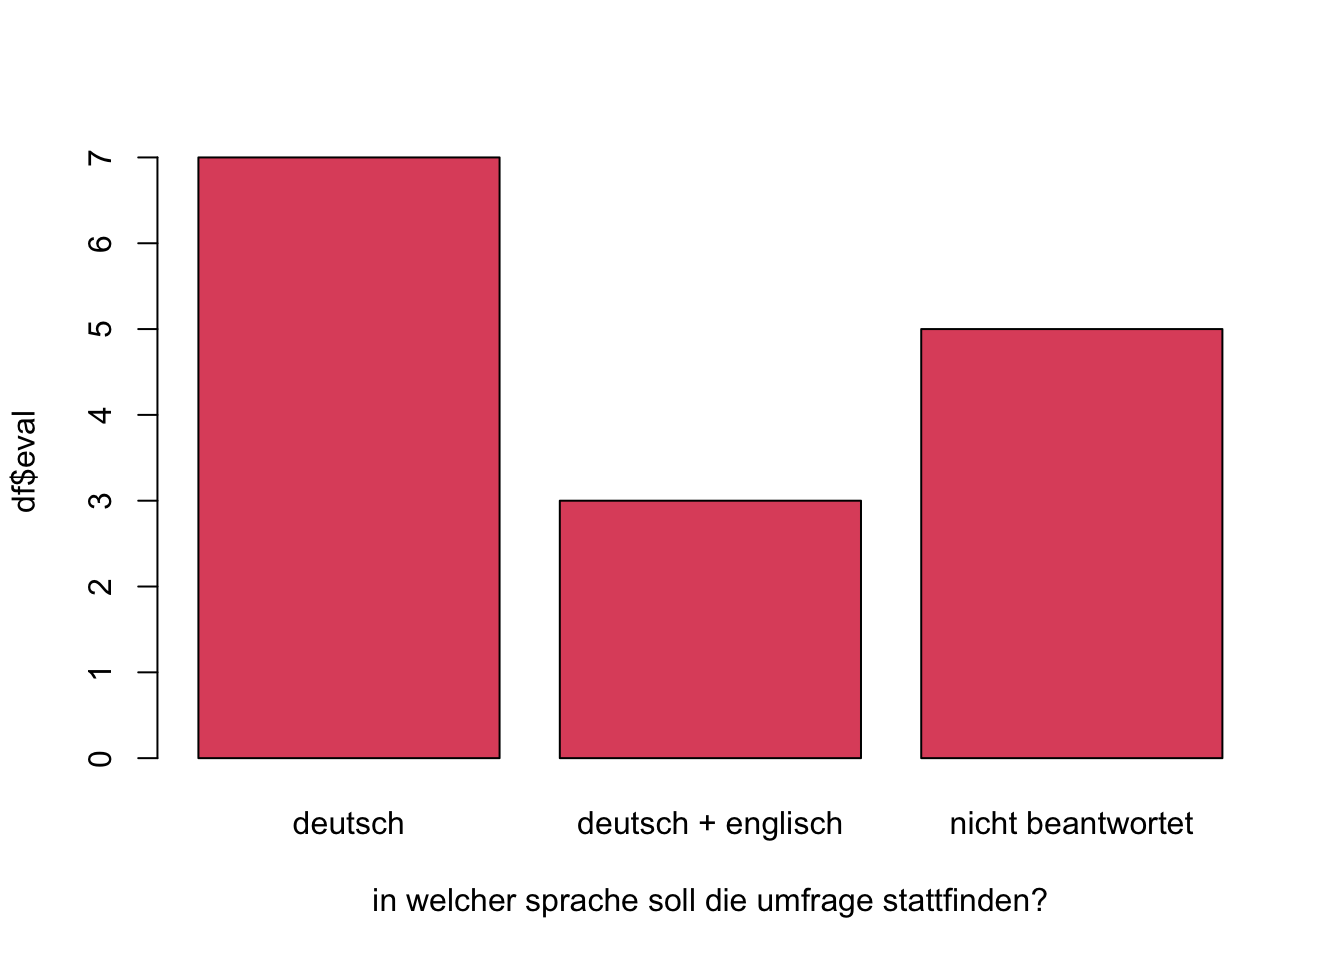
\includegraphics{N-PRG_CA_001pdf_files/figure-latex/unnamed-chunk-3-1.pdf}
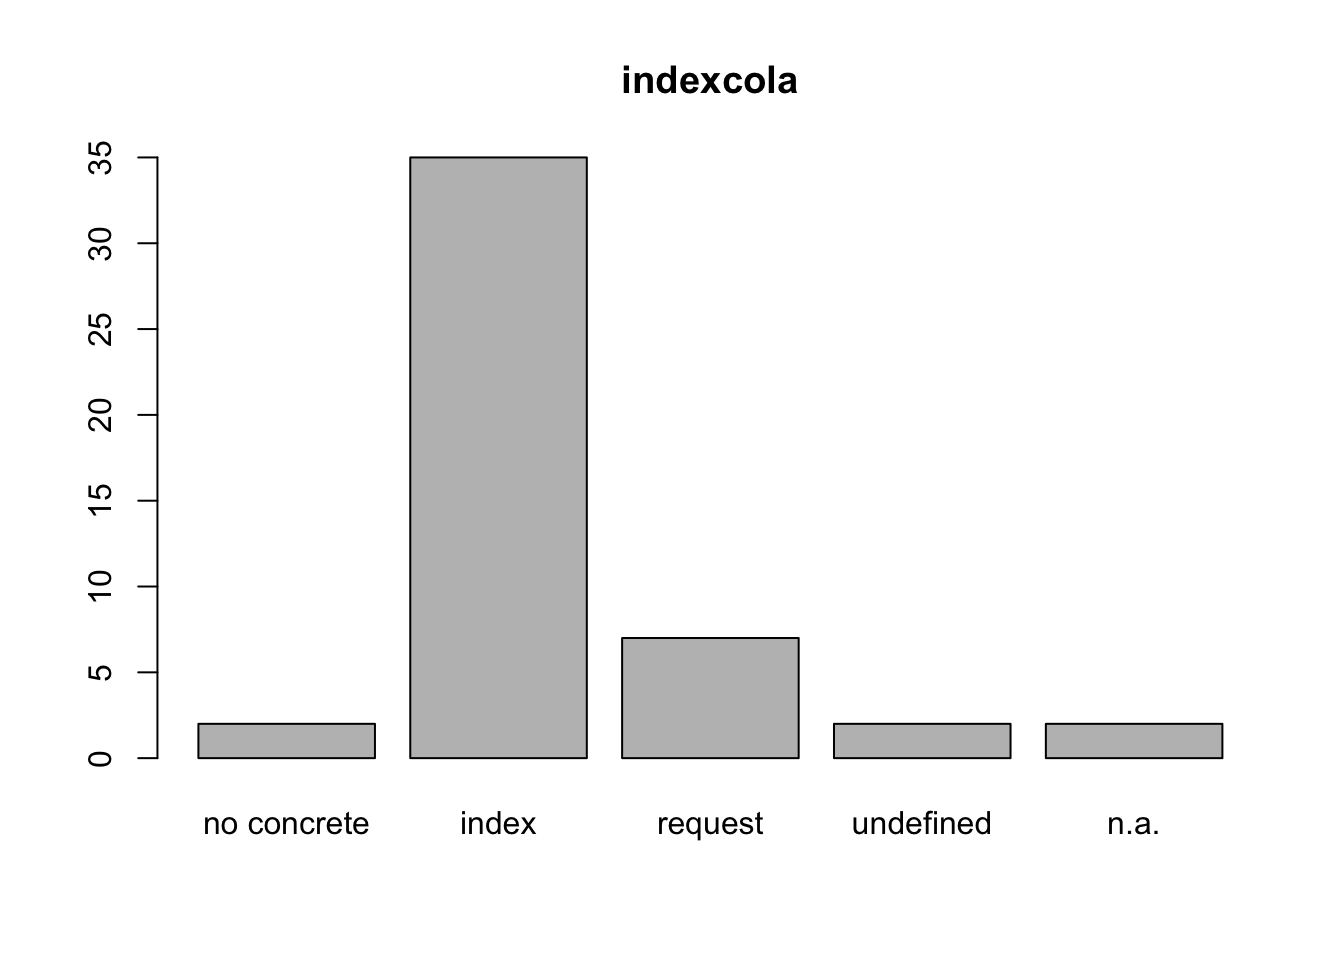
\includegraphics{N-PRG_CA_001pdf_files/figure-latex/unnamed-chunk-3-2.pdf}
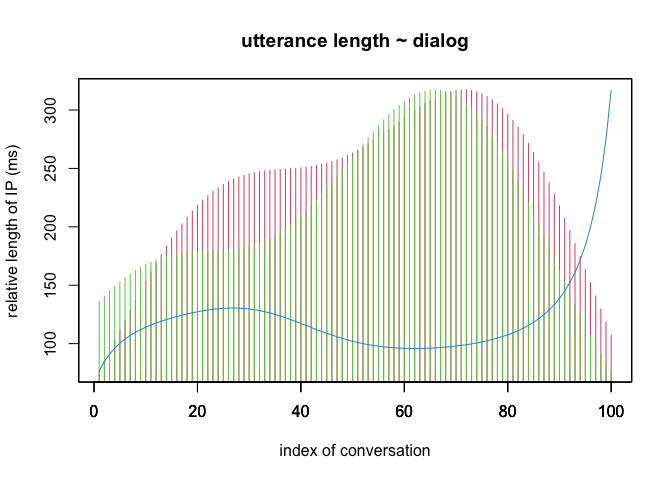
\includegraphics{N-PRG_CA_001pdf_files/figure-latex/unnamed-chunk-3-3.pdf}

Fourier transformation of data cf.~``syuzhet'' R-Package:
\href{https://www.matthewjockers.net/2015/02/02/syuzhet/}{(Jockers
2015)}

\hypertarget{some-numbers}{%
\subsubsection{3.2 some numbers}\label{some-numbers}}

\begin{verbatim}
##     speechacts speech time (sec)  words
## SP0         70                 80   167
## SP1         43                 51    71
\end{verbatim}

\begin{center}\rule{0.5\linewidth}{0.5pt}\end{center}

\hypertarget{a.-notes}{%
\subsection{A. notes}\label{a.-notes}}

\hypertarget{b.-ref}{%
\subsection{B. REF:}\label{b.-ref}}

\hypertarget{refs}{}
\begin{CSLReferences}{1}{0}
\leavevmode\vadjust pre{\hypertarget{ref-elan_elan_2022}{}}%
ELAN. 2022. {``{ELAN} ({Version} 6.4) {[}{Computer} Software{]}.''}
\url{https://archive.mpi.nl/tla/elan}.

\leavevmode\vadjust pre{\hypertarget{ref-jockers_revealing_2015}{}}%
Jockers, Matthew L. 2015. {``Revealing {Sentiment} and {Plot} {Arcs}
with the {Syuzhet} {Package} {Matthew} {L}. {Jockers}.''}
\url{https://www.matthewjockers.net/2015/02/02/syuzhet/}.

\leavevmode\vadjust pre{\hypertarget{ref-worner_exmaralda_2014}{}}%
Wörner, K., and T. Schmidt. 2014. {``{EXMARaLDA}.''} In \emph{Handbook
on {Corpus} {Phonology}}, 402--19. Oxford University Press.
\url{https://exmaralda.org/de/}.

\end{CSLReferences}

\hypertarget{c.-annex}{%
\subsection{C. annex}\label{c.-annex}}

transcript files, tables \& source code:

\end{document}
